% !TEX TS-program = pdflatex
% !TEX encoding = UTF-8 Unicode

% This is a simple template for a LaTeX document using the "article" class.
% See "book", "report", "letter" for other types of document.

\documentclass[8pt]{article} % use larger type; default would be 10pt

\usepackage[utf8]{inputenc} % set input encoding (not needed with XeLaTeX)
\usepackage{bchart}
\usepackage{longtable}
\usepackage{pgfgantt}
\usepackage{calendar} % Use the calendar.sty style
\usepackage{calc}
\usepackage{ifthen}
\usepackage{tkz-base}
\usepackage{pdfpages}
\usepackage{hyperref}
\usepackage{pgfplots}
\usepackage{tkz-kiviat,numprint,fullpage} 
\usepackage{pgfplotstable} 
\usetikzlibrary{arrows}

%%% Examples of Article customizations
% These packages are optional, depending whether you want the features they provide.
% See the LaTeX Companion or other references for full information.

\usepackage{textcomp}
%\usepackage{hyperref}

%%% PAGE DIMENSIONS
\usepackage{geometry} % to change the page dimensions
\geometry{a4paper} % or letterpaper (US) or a5paper or....
% \geometry{margin=2in} % for example, change the margins to 2 inches all round
% \geometry{landscape} % set up the page for landscape
%   read geometry.pdf for detailed page layout information

\usepackage{graphicx} % support the \includegraphics command and options

% \usepackage[parfill]{parskip} % Activate to begin paragraphs with an empty line rather than an indent

%%% PACKAGES
\usepackage{booktabs} % for much better looking tables
\usepackage{array} % for better arrays (eg matrices) in maths
\usepackage{paralist} % very flexible & customisable lists (eg. enumerate/itemize, etc.)
\usepackage{verbatim} % adds environment for commenting out blocks of text & for better verbatim
\usepackage{subfig} % make it possible to include more than one captioned figure/table in a single float
% These packages are all incorporated in the memoir class to one degree or another...

%%% HEADERS & FOOTERS
\usepackage{fancyhdr} % This should be set AFTER setting up the page geometry
\pagestyle{fancy} % options: empty , plain , fancy
\renewcommand{\headrulewidth}{0pt} % customise the layout...
\lhead{}\chead{}\rhead{}
\lfoot{}\cfoot{\thepage}\rfoot{}

%%% SECTION TITLE APPEARANCE
\usepackage{sectsty}
\allsectionsfont{\sffamily\mdseries\upshape} % (See the fntguide.pdf for font help)
% (This matches ConTeXt defaults)

%%% ToC (table of contents) APPEARANCE
\usepackage[nottoc,notlof,notlot]{tocbibind} % Put the bibliography in the ToC
\usepackage[titles,subfigure]{tocloft} % Alter the style of the Table of Contents
\renewcommand{\cftsecfont}{\rmfamily\mdseries\upshape}
\renewcommand{\cftsecpagefont}{\rmfamily\mdseries\upshape} % No bold!

%%% END Article customizations

%%% The "real" document content comes below...

%\includegraphics[width=.2\textwidth]{Logo.png}

\title{Finance}
\author{\copyright Frederic Kerdraon}
%\date{} % Activate to display a given date or no date (if empty),
         % otherwise the current date is printed 

\begin{document}
\maketitle
\tableofcontents

\section{Introduction}

%This document summurizes all the important informations necessary to facilitate things and remove a lot of stress. It's been put together thanks to \LaTeX. This is designed to help make optimal decisions for a not so short lifetime.

{\footnotesize
%Ce n'est pas parceque les choses sont difficiles que nous n'osons pas, c'est parceque nous n'osons pas qu'elles sont difficiles.
}
%\makebox[2\width]{hello}

\newcounter{a}
\newcounter{b}
%----------------------------------------------------------
\newcommand{\slice}[4]{
  \pgfmathparse{0.5*#1+0.5*#2}
  \let\midangle\pgfmathresult

   slice
  \draw[thick,fill=black!10] (0,0) -- (#1:1) arc (#1:#2:1) -- cycle;

   outer label
  \node[label=\midangle:#4] at (\midangle:1) {};

   inner label
  \pgfmathparse{min((#2-#1-10)/110*(-0.3),0)}
  \let\temp\pgfmathresult
  \pgfmathparse{max(\temp,-0.5) + 0.9}
  \let\innerpos\pgfmathresult
  \node at (\midangle:\innerpos) {#3};
}

\section{Management summary}


\subsection{PnL Projections}

{\footnotesize
%Le nombre de simulations est egal au nombre d'arrangements des targets\\
%Pour 8 target, il devrait y avoir un 8! scenarios\\
%Les scenarios sont ordonnes par facilite de mise en oeuvre min(complexity, cost,etc)\\

\subsubsection{Latex Graph of the scenarios}

$TotalDrift = 0.01;\\
$TotalScenTox = 0;\\
$TotalScenDebt = 0;\\
$TotalScenCash = 0;\\
$TotalScenToxDebt = 0;\\
$TotalScen = 0;\\
$Scen = 135;\\
$ScenToxics = 231;\\
$ScenDebt = 529*.4;\\
$ScenCash = 755*.5;\\
$ScenToxDebt = 231+529*.4;\\

my @Scen = (231,529*.4,755*.5,231+529*.4,1000,700,800,950,750);\\

\setlength{\unitlength}{1cm}
\begin{picture}(12,11)(0,0)
\put(0,0){\vector(1,0){12.1}}
\put(12,-.35){$Month$}
\put(0,-6){\vector(0,1){12}}
\put(0,6.5){\makebox(0,0){$PnL$)}}
\put( -0.5,1){$1$}
\put( -0.5,2){$2$}
\put( -0.5,3){$3$}
\put( -0.5,4){$4$}
\put( -0.5,5){$5$}
\put( -0.5,6){$6$}
\put( -0.5,-1){$-1$}
\put( -0.5,-2){$-2$}
\put( -0.5,-3){$-3$}
\put( -0.5,-4){$-4$}
\put( -0.5,-5){$-5$}
\put( -0.5,-6){$-6$}
\qbezier(0.0,0.0)(1.2384,0.0)(2.0,2.7622)
\linethickness{.090mm}
\put( 0,6){$1$}
\put( 0,0.472810){\line(2,0){.2}}
\put( 0,0){\line(0,1){0.472810}}
\put( 0.2,0){\line(0,1){0.472810}}
\put( 0,0.572810){$Scen0$}
\put( 0,0.703810){\line(2,0){.5}}
\put( 0,0){\line(0,1){0.703810}}
\put( 0.5,0){\line(0,1){0.703810}}
\put( 0,0.684410){\line(2,0){.5}}
\put( 0,0){\line(0,1){0.684410}}
\put( 0.5,0){\line(0,1){0.684410}}
\put( 1,6){$2$}
\put( 1,-0.002590){\line(2,0){.2}}
\put( 1,-0.002590){\line(0,1){0.002590}}
\put( 1.2,-0.002590){\line(0,1){0.002590}}
\put( 1,-0.302590){$Scen0$}
\put( 1,0.459410){\line(2,0){.5}}
\put( 1,0){\line(0,1){0.459410}}
\put( 1.5,0){\line(0,1){0.459410}}
\put( 1,0.420610){\line(2,0){.5}}
\put( 1,0){\line(0,1){0.420610}}
\put( 1.5,0){\line(0,1){0.420610}}
\end{picture}


\subsubsection{Plot of an example}
\includegraphics[scale=0.3]{Finance.png}}

%\subsubsection{Latex example}
%\input{parabola-plot}

%\subsubsection{Latex example}
%\input{tikzdevice-demo}

%\subsubsection{Latex example}
%\input{TimeTable}

%\subsubsection{Latex example}
%\input{Torn Paper}

%\subsubsection{Latex example}
%\input{Weather Table}

%\subsubsection{Latex example}
%

\documentclass[a5paper]{article}

% Requires PGF >=  1.09
% Note:
%   This example works only with pdftex >= 1.30.0
%   You have to run pdftex on the example twice!
\usepackage{amsmath}
\usepackage{tikz}

\begin{document}
\thispagestyle{empty}

Lorem ipsum dolor sit amet, consectetuer adipiscing elit. Donec luctus 
mollis nisl. Nullam tempor, diam non tincidunt tincidunt, nunc tortor 
elementum odio, nec iaculis urna leo a eros. Lorem ipsum dolor sit amet,
consectetuer adipiscing elit. Sed elit elit, pellentesque et, 
sollicitudin a, imperdiet eget, tellus. Vestibulum et sapien. Maecenas 
libero. Vivamus vel metus in ipsum ultricies commodo. Donec quam. Fusce 
arcu. In est felis, sagittis vitae, vehicula ut, tristique vitae, eros. 
Mauris ut lorem vel risus posuere elementum. Quisque volutpat ornare lorem. 
Integer porta.
\begin{multline}\label{eq:steeringfull}
    \begin{bmatrix}
        m-Y_{\dot{v}} & Y_{\dot{r}} & 0\\
        -N_{\dot{v}} & I_z-N_{\dot{r}} & 0\\
        0 & 0 & 1
    \end{bmatrix}
    \begin{bmatrix}
        \dot{v} \\ \dot{r}\\ \dot{\psi}
    \end{bmatrix}\\ +
    \begin{bmatrix}
        -Y_v & -Y_r+mu_0\\
        -N_v & -N_r & 0\\
        0 & -1 & 0
    \end{bmatrix}
    \begin{bmatrix}
        v \\ r \\ \psi
    \end{bmatrix} =
    \begin{bmatrix}
        Y_\delta \\ N_\delta \\ 0
    \end{bmatrix}\delta_r
\end{multline}

Donec ut neque vel leo sagittis tristique. Cras et justo. Mauris lorem 
purus, sagittis eu, consectetuer et, lacinia et, augue. Ut in velit in 
diam semper rutrum. Nunc rhoncus. Cras tincidunt. Aenean nec quam. In commodo
sem ac nulla. Donec fermentum metus non nisl sagittis sagittis. Vestibulum 
sit amet nunc. Vivamus dapibus congue purus. Quisque arcu tellus, 
pellentesque ac, tincidunt lobortis, commodo ac, purus.


% Start of the interesting part
% If you place the code at the beginning of the page, the image will be
% put behind the text.
%
% The overlay option removes the picture from the ordinary page flow. 
\begin{tikzpicture}[remember picture, overlay]
    \node[inner sep=0pt] at (current page.center) {%
        \includegraphics[width=\paperwidth,height=\paperheight]{007}%
    };%
\end{tikzpicture}


\end{document}



%\subsubsection{Latex example}
%\input{}
%\subsubsection{Latex example}
%\input{}
%\subsubsection{Latex example}
%\input{}
%\subsubsection{Latex example}
%\input{}

\subsubsection{Plot of an example}
\includegraphics[scale=0.3]{Finance.png}}

On the graph we can notice that all the scenarios are positive, as they were built to show how to maximize profit
just by managing the charge, and especially useless charges.\\
\subsubsection{Graph}
\includegraphics[scale=0.5]{Vector.png}}

%\includepdf[pages={1}]{stockchart.pdf}
%\includepdf[pages={1}]{friedberg.pdf}
\subsubsection{Surface}
\begin{tikzpicture}
\begin{axis}
\addplot[color=red]{exp(x)};
\end{axis}
\end{tikzpicture}
%Here ends the furst plot
\hskip 5pt
%Here begins the 3d plot
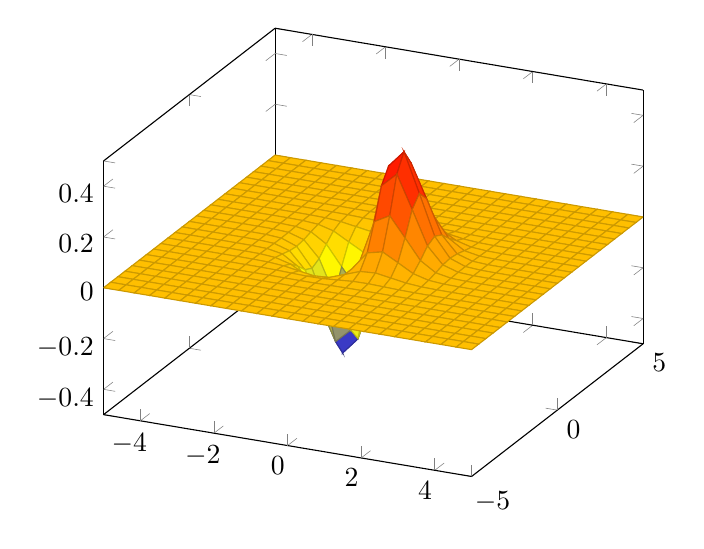
\begin{tikzpicture}
\begin{axis}
\addplot3[
    surf,
]
{exp(-x^2-y^2)*x};
\end{axis}
\end{tikzpicture}

This surface is really good looking but I doubt on its information.\\
\subsubsection{Table}
The scenarios given in the table are only examples, the real scenarios are provided in the graph below
\begin{longtable}{|c|c|c|c|c|c|}
\hline
\multicolumn{6}{|c|}{Scenarios} \\
\hline
PnL; CumPnL; Tox; Debt(40%); Cash(50%); Tox-Debt(40%)
PnL & CumPnL & Tox & Debt(40\%) & Cash(50\%) & Tox-Debt(40\%)
\hline
-475;-475;-244;-263;-97;-32
-475 & -475 & -244 & -263 & -97 & -32\\
\hline
140;-335;126;87;419;549
140 & -335 & 126 & 87 & 419 & 549\\
\hline
136;-199;493;435;933;1128
136 & -199 & 493 & 435 & 933 & 1128\\
\hline
122;-77;846;769;1432;1693
122 & -77 & 846 & 769 & 1432 & 1693\\
\hline
82;5;1160;1063;1892;2218
82 & 5 & 1160 & 1063 & 1892 & 2218\\
\hline
70;75;1461;1345;2340;2731
70 & 75 & 1461 & 1345 & 2340 & 2731\\
\hline
63;139;1756;1620;2781;3237
63 & 139 & 1756 & 1620 & 2781 & 3237\\
\hline
43;182;2030;1874;3202;3722
43 & 182 & 2030 & 1874 & 3202 & 3722\\
\hline
37;219;2298;2123;3616;4202
37 & 219 & 2298 & 2123 & 3616 & 4202\\
\hline
-18;200;2510;2316;3975;4626
-18 & 200 & 2510 & 2316 & 3975 & 4626\\
\hline
\end{longtable}

All the figures need to be checked carefully by someone who knows what it's doing.
}

\subsection{History and extrapolations}

\subsubsection{Kapital curve}
Kapital trend,Assets trend,Liabilities trend,Leverage trend\\
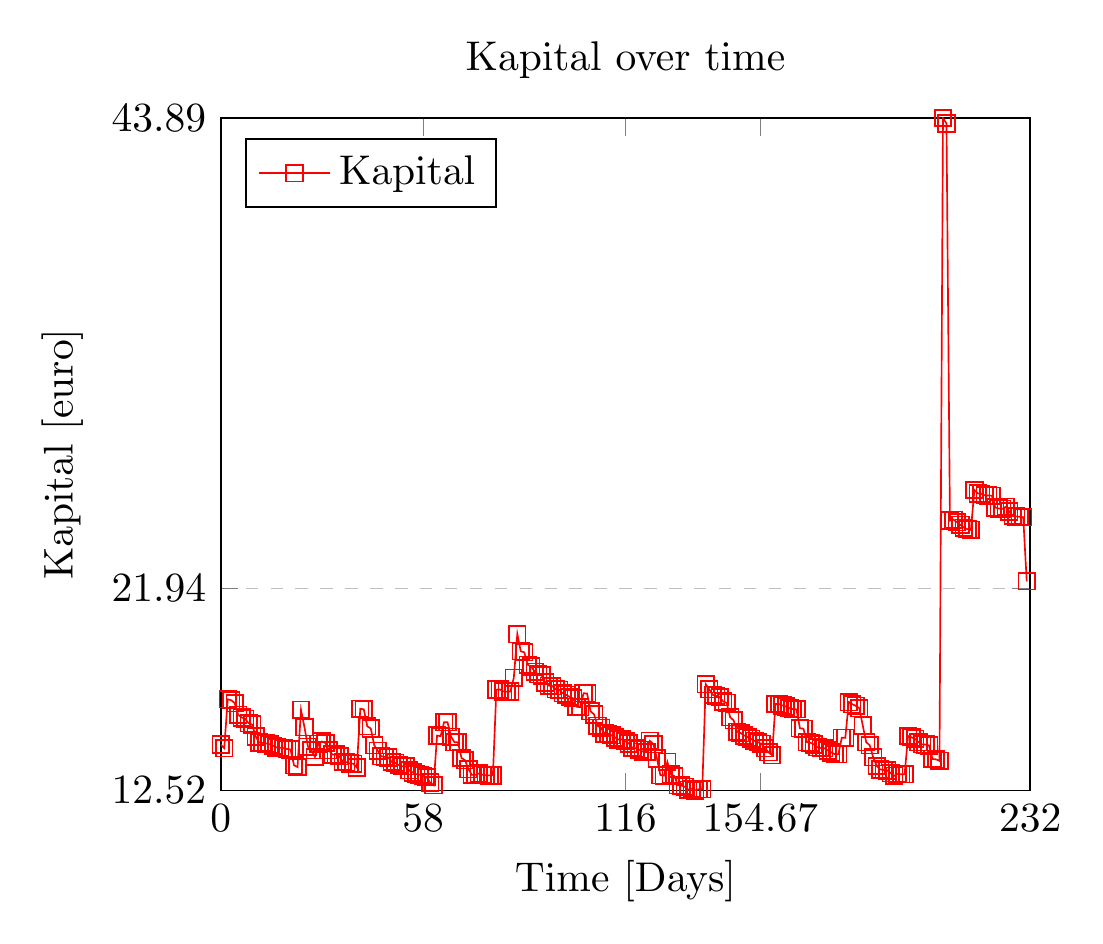
\begin{tikzpicture}[thick, scale=1.5]
\begin{axis}[
title={Kapital over time},
xlabel={Time [Days]},
ylabel={Kapital [euro]},
xmin=0,xmax=232,
ymin=12.515,ymax=43.885,
xtick={0,58,116,154.666666666667,232},
ytick={12.515,6.2575,0,21.9425,43.885},
legend pos=north west,
ymajorgrids=true,
grid style=dashed,
]
\addplot[
color=red,
mark=square,
]
coordinates {
(0,14.653)(1,14.488)(2,16.766)(3,16.726)(4,16.589)(5,16.042)(6,15.923)(7,15.856)(8,15.651)(9,15.59)(10,15.037)(11,14.751)(12,14.733)(13,14.708)(14,14.673)(15,14.603)(16,14.525)(17,14.505)(18,14.491)(19,14.448)(20,14.428)(21,13.693)(22,13.609)(23,16.276)(24,15.46)(25,14.556)(26,14.398)(27,14.076)(28,14.698)(29,14.803)(30,14.729)(31,14.39)(32,14.191)(33,14.191)(34,14.111)(35,13.856)(36,13.832)(37,13.772)(38,13.763)(39,13.586)(40,16.325)(41,16.298)(42,15.507)(43,15.406)(44,14.628)(45,14.37)(46,14.116)(47,14.08)(48,14.057)(49,13.846)(50,13.802)(51,13.702)(52,13.647)(53,13.647)(54,13.453)(55,13.357)(56,13.277)(57,13.252)(58,13.202)(59,13.142)(60,12.888)(61,12.761)(62,15.079)(63,15.046)(64,15.696)(65,15.696)(66,15.026)(67,14.764)(68,14.76)(69,14.029)(70,13.931)(71,13.508)(72,13.24)(73,13.242)(74,13.306)(75,13.248)(76,13.225)(77,13.219)(78,13.219)(79,17.219)(80,17.229)(81,17.137)(82,17.123)(83,17.128)(84,17.778)(85,19.812)(86,19.007)(87,18.958)(88,18.381)(89,18.293)(90,18.054)(91,17.934)(92,17.874)(93,17.549)(94,17.405)(95,17.385)(96,17.235)(97,17.215)(98,17.057)(99,16.977)(100,16.876)(101,16.812)(102,16.417)(103,16.402)(104,17.052)(105,17.036)(106,16.207)(107,16.061)(108,15.528)(109,15.433)(110,15.175)(111,15.159)(112,15.086)(113,14.99)(114,14.89)(115,14.89)(116,14.81)(117,14.706)(118,14.499)(119,14.487)(120,14.412)(121,14.326)(122,14.308)(123,14.829)(124,14.678)(125,14.008)(126,13.233)(127,13.205)(128,13.847)(129,13.258)(130,13.19)(131,12.757)(132,12.747)(133,12.687)(134,12.551)(135,12.597)(136,12.515)(137,12.573)(138,12.573)(139,17.473)(140,17.239)(141,16.974)(142,16.928)(143,16.867)(144,16.663)(145,16.602)(146,15.929)(147,15.785)(148,15.256)(149,15.194)(150,15.083)(151,15.007)(152,14.917)(153,14.827)(154,14.765)(155,14.685)(156,14.484)(157,14.295)(158,14.162)(159,16.547)(160,16.546)(161,16.481)(162,16.43)(163,16.35)(164,16.308)(165,16.299)(166,15.415)(167,15.399)(168,14.772)(169,14.742)(170,14.662)(171,14.53)(172,14.495)(173,14.49)(174,14.384)(175,14.291)(176,14.207)(177,14.199)(178,14.977)(179,14.967)(180,16.639)(181,16.539)(182,16.463)(183,16.357)(184,15.551)(185,14.762)(186,14.627)(187,14.066)(188,13.657)(189,13.499)(190,13.466)(191,13.448)(192,13.327)(193,13.196)(194,13.287)(195,13.272)(196,13.272)(197,15.056)(198,14.996)(199,14.919)(200,14.767)(201,14.666)(202,14.654)(203,14.618)(204,13.984)(205,13.966)(206,13.893)(207,43.885)(208,43.629)(209,25.102)(210,25.145)(211,25.035)(212,24.904)(213,24.775)(214,24.702)(215,24.668)(216,26.531)(217,26.371)(218,26.353)(219,26.283)(220,26.272)(221,26.267)(222,25.715)(223,25.667)(224,25.65)(225,25.749)(226,25.524)(227,25.32)(228,25.3)(229,25.283)(230,25.262)(231,22.271)
};
\legend{Kapital}
\end{axis}
\end{tikzpicture}


\subsubsection{PnL curve}

PnL trend\\
Income trend\\
Expenses trend\\
%\input{pnlCurve}
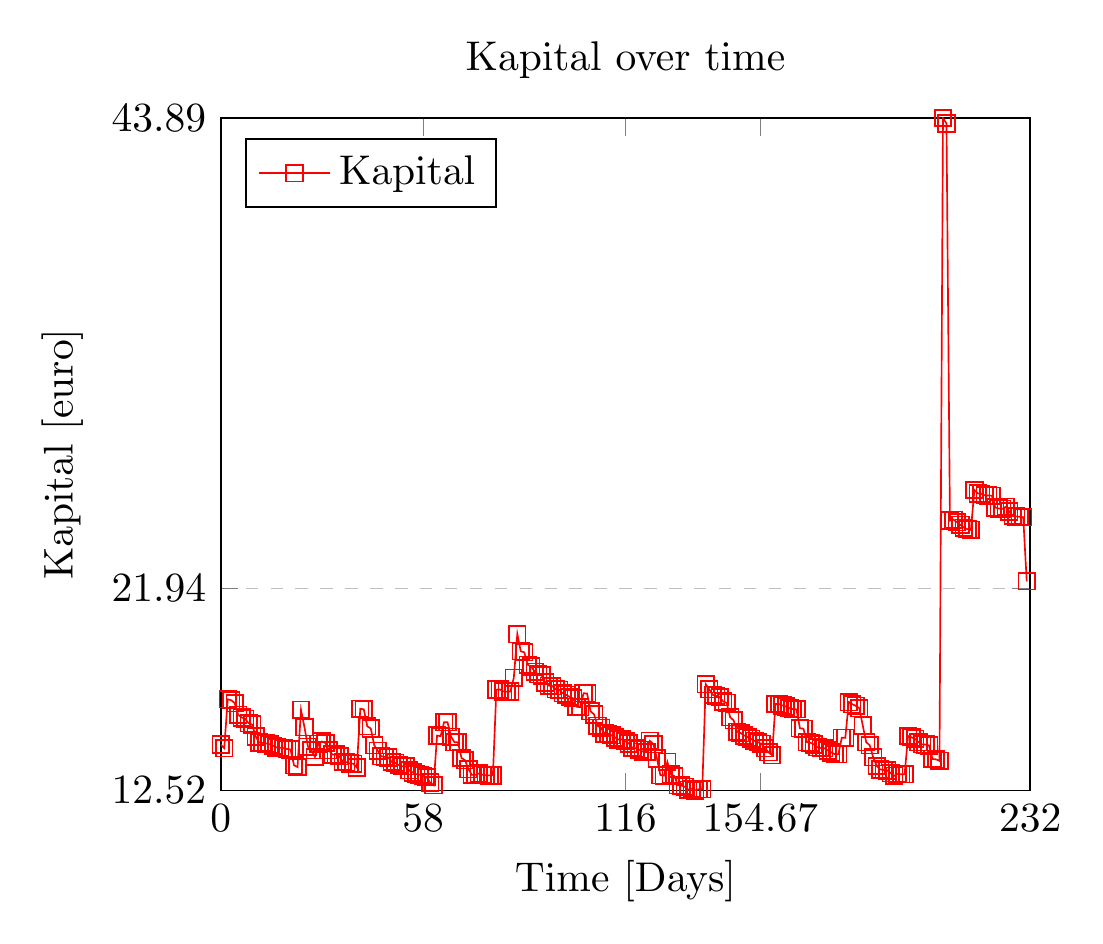
\begin{tikzpicture}[thick, scale=1.5]
\begin{axis}[
title={Kapital over time},
xlabel={Time [Days]},
ylabel={Kapital [euro]},
xmin=0,xmax=232,
ymin=12.515,ymax=43.885,
xtick={0,58,116,154.666666666667,232},
ytick={12.515,6.2575,0,21.9425,43.885},
legend pos=north west,
ymajorgrids=true,
grid style=dashed,
]
\addplot[
color=red,
mark=square,
]
coordinates {
(0,14.653)(1,14.488)(2,16.766)(3,16.726)(4,16.589)(5,16.042)(6,15.923)(7,15.856)(8,15.651)(9,15.59)(10,15.037)(11,14.751)(12,14.733)(13,14.708)(14,14.673)(15,14.603)(16,14.525)(17,14.505)(18,14.491)(19,14.448)(20,14.428)(21,13.693)(22,13.609)(23,16.276)(24,15.46)(25,14.556)(26,14.398)(27,14.076)(28,14.698)(29,14.803)(30,14.729)(31,14.39)(32,14.191)(33,14.191)(34,14.111)(35,13.856)(36,13.832)(37,13.772)(38,13.763)(39,13.586)(40,16.325)(41,16.298)(42,15.507)(43,15.406)(44,14.628)(45,14.37)(46,14.116)(47,14.08)(48,14.057)(49,13.846)(50,13.802)(51,13.702)(52,13.647)(53,13.647)(54,13.453)(55,13.357)(56,13.277)(57,13.252)(58,13.202)(59,13.142)(60,12.888)(61,12.761)(62,15.079)(63,15.046)(64,15.696)(65,15.696)(66,15.026)(67,14.764)(68,14.76)(69,14.029)(70,13.931)(71,13.508)(72,13.24)(73,13.242)(74,13.306)(75,13.248)(76,13.225)(77,13.219)(78,13.219)(79,17.219)(80,17.229)(81,17.137)(82,17.123)(83,17.128)(84,17.778)(85,19.812)(86,19.007)(87,18.958)(88,18.381)(89,18.293)(90,18.054)(91,17.934)(92,17.874)(93,17.549)(94,17.405)(95,17.385)(96,17.235)(97,17.215)(98,17.057)(99,16.977)(100,16.876)(101,16.812)(102,16.417)(103,16.402)(104,17.052)(105,17.036)(106,16.207)(107,16.061)(108,15.528)(109,15.433)(110,15.175)(111,15.159)(112,15.086)(113,14.99)(114,14.89)(115,14.89)(116,14.81)(117,14.706)(118,14.499)(119,14.487)(120,14.412)(121,14.326)(122,14.308)(123,14.829)(124,14.678)(125,14.008)(126,13.233)(127,13.205)(128,13.847)(129,13.258)(130,13.19)(131,12.757)(132,12.747)(133,12.687)(134,12.551)(135,12.597)(136,12.515)(137,12.573)(138,12.573)(139,17.473)(140,17.239)(141,16.974)(142,16.928)(143,16.867)(144,16.663)(145,16.602)(146,15.929)(147,15.785)(148,15.256)(149,15.194)(150,15.083)(151,15.007)(152,14.917)(153,14.827)(154,14.765)(155,14.685)(156,14.484)(157,14.295)(158,14.162)(159,16.547)(160,16.546)(161,16.481)(162,16.43)(163,16.35)(164,16.308)(165,16.299)(166,15.415)(167,15.399)(168,14.772)(169,14.742)(170,14.662)(171,14.53)(172,14.495)(173,14.49)(174,14.384)(175,14.291)(176,14.207)(177,14.199)(178,14.977)(179,14.967)(180,16.639)(181,16.539)(182,16.463)(183,16.357)(184,15.551)(185,14.762)(186,14.627)(187,14.066)(188,13.657)(189,13.499)(190,13.466)(191,13.448)(192,13.327)(193,13.196)(194,13.287)(195,13.272)(196,13.272)(197,15.056)(198,14.996)(199,14.919)(200,14.767)(201,14.666)(202,14.654)(203,14.618)(204,13.984)(205,13.966)(206,13.893)(207,43.885)(208,43.629)(209,25.102)(210,25.145)(211,25.035)(212,24.904)(213,24.775)(214,24.702)(215,24.668)(216,26.531)(217,26.371)(218,26.353)(219,26.283)(220,26.272)(221,26.267)(222,25.715)(223,25.667)(224,25.65)(225,25.749)(226,25.524)(227,25.32)(228,25.3)(229,25.283)(230,25.262)(231,22.271)
};
\legend{Kapital}
\end{axis}
\end{tikzpicture}


\subsubsection{Cash curve}

Funny cashflow/kapital superior to percent\\

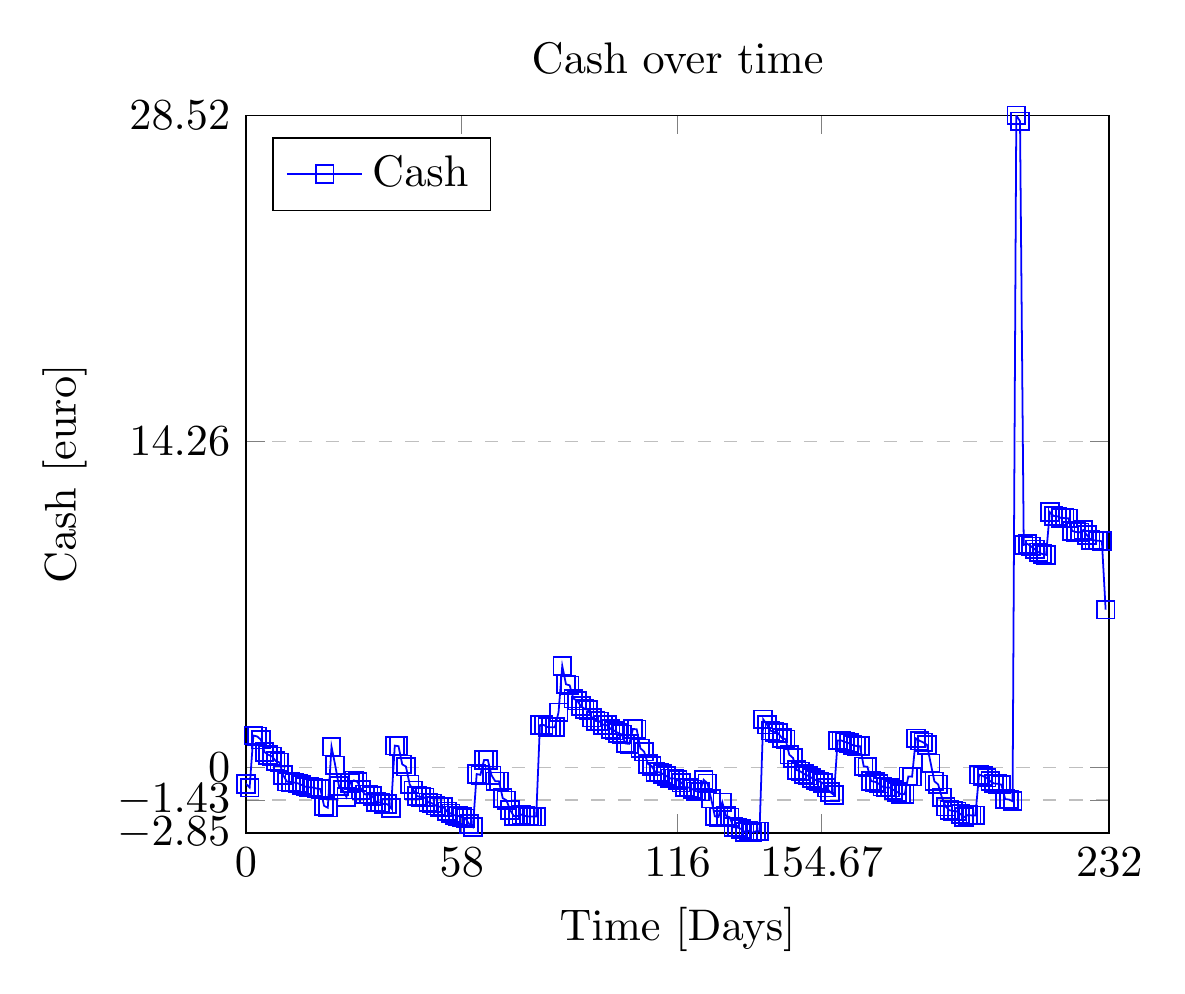
\begin{tikzpicture}[thick, scale=1.6]
\begin{axis}[
title={Cash over time},
xlabel={Time [Days]},
ylabel={Cash [euro]},
xmin=0,xmax=232,
ymin=-2.851,ymax=28.519,
xtick={0,58,116,154.666666666667,232},
ytick={-2.851,-1.4255,0,14.2595,28.519},
legend pos=north west,
ymajorgrids=true,
grid style=dashed,
]
\addplot[
color=blue,
mark=square,
]
coordinates {
(0,-0.713)(1,-0.878)(2,1.4)(3,1.36)(4,1.223)(5,0.676)(6,0.557)(7,0.49)(8,0.285)(9,0.224)(10,-0.329)(11,-0.615)(12,-0.633)(13,-0.658)(14,-0.693)(15,-0.763)(16,-0.841)(17,-0.861)(18,-0.875)(19,-0.918)(20,-0.938)(21,-1.673)(22,-1.757)(23,0.91)(24,0.094)(25,-0.81)(26,-0.968)(27,-1.29)(28,-0.668)(29,-0.563)(30,-0.637)(31,-0.976)(32,-1.175)(33,-1.175)(34,-1.255)(35,-1.51)(36,-1.534)(37,-1.594)(38,-1.603)(39,-1.78)(40,0.959)(41,0.932)(42,0.141)(43,0.04)(44,-0.738)(45,-0.996)(46,-1.25)(47,-1.286)(48,-1.309)(49,-1.52)(50,-1.564)(51,-1.664)(52,-1.719)(53,-1.719)(54,-1.913)(55,-2.009)(56,-2.089)(57,-2.114)(58,-2.164)(59,-2.224)(60,-2.478)(61,-2.605)(62,-0.287)(63,-0.32)(64,0.33)(65,0.33)(66,-0.34)(67,-0.602)(68,-0.606)(69,-1.337)(70,-1.435)(71,-1.858)(72,-2.126)(73,-2.124)(74,-2.06)(75,-2.118)(76,-2.141)(77,-2.147)(78,-2.147)(79,1.853)(80,1.863)(81,1.771)(82,1.757)(83,1.762)(84,2.412)(85,4.446)(86,3.641)(87,3.592)(88,3.015)(89,2.927)(90,2.688)(91,2.568)(92,2.508)(93,2.183)(94,2.039)(95,2.019)(96,1.869)(97,1.849)(98,1.691)(99,1.611)(100,1.51)(101,1.446)(102,1.051)(103,1.036)(104,1.686)(105,1.67)(106,0.841)(107,0.695)(108,0.162)(109,0.067)(110,-0.191)(111,-0.207)(112,-0.28)(113,-0.376)(114,-0.476)(115,-0.476)(116,-0.556)(117,-0.66)(118,-0.867)(119,-0.879)(120,-0.954)(121,-1.04)(122,-1.058)(123,-0.537)(124,-0.688)(125,-1.358)(126,-2.133)(127,-2.161)(128,-1.519)(129,-2.108)(130,-2.176)(131,-2.609)(132,-2.619)(133,-2.679)(134,-2.815)(135,-2.769)(136,-2.851)(137,-2.793)(138,-2.793)(139,2.107)(140,1.873)(141,1.608)(142,1.562)(143,1.501)(144,1.297)(145,1.236)(146,0.563)(147,0.419)(148,-0.11)(149,-0.172)(150,-0.283)(151,-0.359)(152,-0.449)(153,-0.539)(154,-0.601)(155,-0.681)(156,-0.882)(157,-1.071)(158,-1.204)(159,1.181)(160,1.18)(161,1.115)(162,1.064)(163,0.984)(164,0.942)(165,0.933)(166,0.049)(167,0.033)(168,-0.594)(169,-0.624)(170,-0.704)(171,-0.836)(172,-0.871)(173,-0.876)(174,-0.982)(175,-1.075)(176,-1.159)(177,-1.167)(178,-0.389)(179,-0.399)(180,1.273)(181,1.173)(182,1.097)(183,0.991)(184,0.185)(185,-0.604)(186,-0.739)(187,-1.3)(188,-1.709)(189,-1.867)(190,-1.9)(191,-1.918)(192,-2.039)(193,-2.17)(194,-2.079)(195,-2.094)(196,-2.094)(197,-0.31)(198,-0.37)(199,-0.447)(200,-0.599)(201,-0.7)(202,-0.712)(203,-0.748)(204,-1.382)(205,-1.4)(206,-1.473)(207,28.519)(208,28.263)(209,9.736)(210,9.779)(211,9.669)(212,9.538)(213,9.409)(214,9.336)(215,9.302)(216,11.165)(217,11.005)(218,10.987)(219,10.917)(220,10.906)(221,10.901)(222,10.349)(223,10.301)(224,10.284)(225,10.383)(226,10.158)(227,9.954)(228,9.934)(229,9.917)(230,9.896)(231,6.905)
};
\legend{Cash}
\end{axis}
\end{tikzpicture}

%Checklists.tex:%\includegraphics[scale=0.5]{stockchart.pdf}}

\section{Cash Balance Management}

\subsection{Monthly drift}

{\footnotesize
Data are aggregated between Initial date: \textbf{2011/01/01} and Last date: \textbf{2021-01-13}

}

\subsubsection{Table}
\input{almGraph}

\footnotesize{
\subsubsection{Table}
\begin{longtable}{|c|c|c|c|c|c|}
\hline
\multicolumn{6}{|c|}{Cashflows} \\
\hline
MinDate & MaxDate & Income & Charges & PnL & NumDays\\
\hline
2011-01-01 & 2021-01-13 & 83303 & 77592 & 5711 & 3665\\
\hline
2011-01-01 & 2016-10-07 & 83303 & 77592 & 5711 & 2106\\
\hline
2011-01-01 & 2016-10-06 & 83303 & 77588 & 5715 & 2105\\
\hline
2011-01-01 & 2016-10-05 & 83303 & 77581 & 5722 & 2104\\
\hline
2011-01-01 & 2016-10-04 & 83303 & 77558 & 5745 & 2103\\
\hline
2011-01-01 & 2016-10-03 & 83303 & 77484 & 5819 & 2102\\
\hline
2011-01-01 & 2016-09-30 & 83303 & 77308 & 5995 & 2099\\
\hline
2011-01-01 & 2016-09-29 & 83303 & 77278 & 6025 & 2098\\
\hline
2011-01-01 & 2016-09-28 & 83303 & 77246 & 6057 & 2097\\
\hline
2011-01-01 & 2016-09-27 & 83303 & 77223 & 6080 & 2096\\
\hline
2011-01-01 & 2016-09-26 & 82027 & 77216 & 4811 & 2095\\
\hline
2011-01-01 & 2016-09-21 & 82027 & 77134 & 4893 & 2090\\
\hline
2011-01-01 & 2016-09-20 & 82027 & 77044 & 4983 & 2089\\
\hline
2011-01-01 & 2016-09-19 & 82027 & 77018 & 5009 & 2088\\
\hline
2011-01-01 & 2016-09-16 & 82027 & 76951 & 5076 & 2085\\
\hline
 ... & ... & ... & ... & ... & ...\\
\hline
 Total &  &  &  &  & \\
\hline
\end{longtable}

To be able to have data for the drift, you need to build a C++ insert like for the kapital
go through the dates in the cashflows, and calculate a drift based on this (modulo the salary) 
\subsubsection{Graph}
%\includegraphics[width=.8\textwidth]{PnL.png}
%\begin{bchart}[min=0,max=96,step=32,unit=k\texteuro]
\bcbar[label=Income]{96}\\
\smallskip
\bcbar[label=Charges]{92}\\
\smallskip
\bcbar[label=Drift]{4}\\
\smallskip
\bcbar[label=Income]{96}\\
\smallskip
\bcbar[label=Charges]{92}\\
\smallskip
\bcbar[label=Drift]{4}\\
\smallskip
\bcbar[label=Income]{96}\\
\smallskip
\bcbar[label=Charges]{92}\\
\smallskip
\bcbar[label=Drift]{4}\\
\smallskip
\bcbar[label=Income]{96}\\
\smallskip
\bcbar[label=Charges]{92}\\
\smallskip
\bcbar[label=Drift]{4}\\
\smallskip
\bcbar[label=Income]{96}\\
\smallskip
\bcbar[label=Charges]{91}\\
\smallskip
\bcbar[label=Drift]{5}\\
\smallskip
\bcbar[label=Income]{96}\\
\smallskip
\bcbar[label=Charges]{91}\\
\smallskip
\bcbar[label=Drift]{5}\\
\smallskip
\bcbar[label=Income]{96}\\
\smallskip
\bcbar[label=Charges]{91}\\
\smallskip
\bcbar[label=Drift]{5}\\
\smallskip
\bcbar[label=Income]{96}\\
\smallskip
\bcbar[label=Charges]{91}\\
\smallskip
\bcbar[label=Drift]{5}\\
\smallskip
\bcbar[label=Income]{96}\\
\smallskip
\bcbar[label=Charges]{91}\\
\smallskip
\bcbar[label=Drift]{5}\\
\smallskip
\bcbar[label=Income]{96}\\
\smallskip
\bcbar[label=Charges]{91}\\
\smallskip
\bcbar[label=Drift]{5}\\
\smallskip
\bcbar[label=Income]{96}\\
\smallskip
\bcbar[label=Charges]{90}\\
\smallskip
\bcbar[label=Drift]{6}\\
\smallskip
\bcbar[label=Income]{96}\\
\smallskip
\bcbar[label=Charges]{90}\\
\smallskip
\bcbar[label=Drift]{6}\\
\smallskip
\bcbar[label=Income]{96}\\
\smallskip
\bcbar[label=Charges]{90}\\
\smallskip
\bcbar[label=Drift]{6}\\
\smallskip
\bcbar[label=Income]{96}\\
\smallskip
\bcbar[label=Charges]{90}\\
\smallskip
\bcbar[label=Drift]{6}\\
\smallskip
\bcbar[label=Income]{96}\\
\smallskip
\bcbar[label=Charges]{90}\\
\smallskip
\bcbar[label=Drift]{6}\\
\smallskip
\end{bchart}

%\input{Plot}
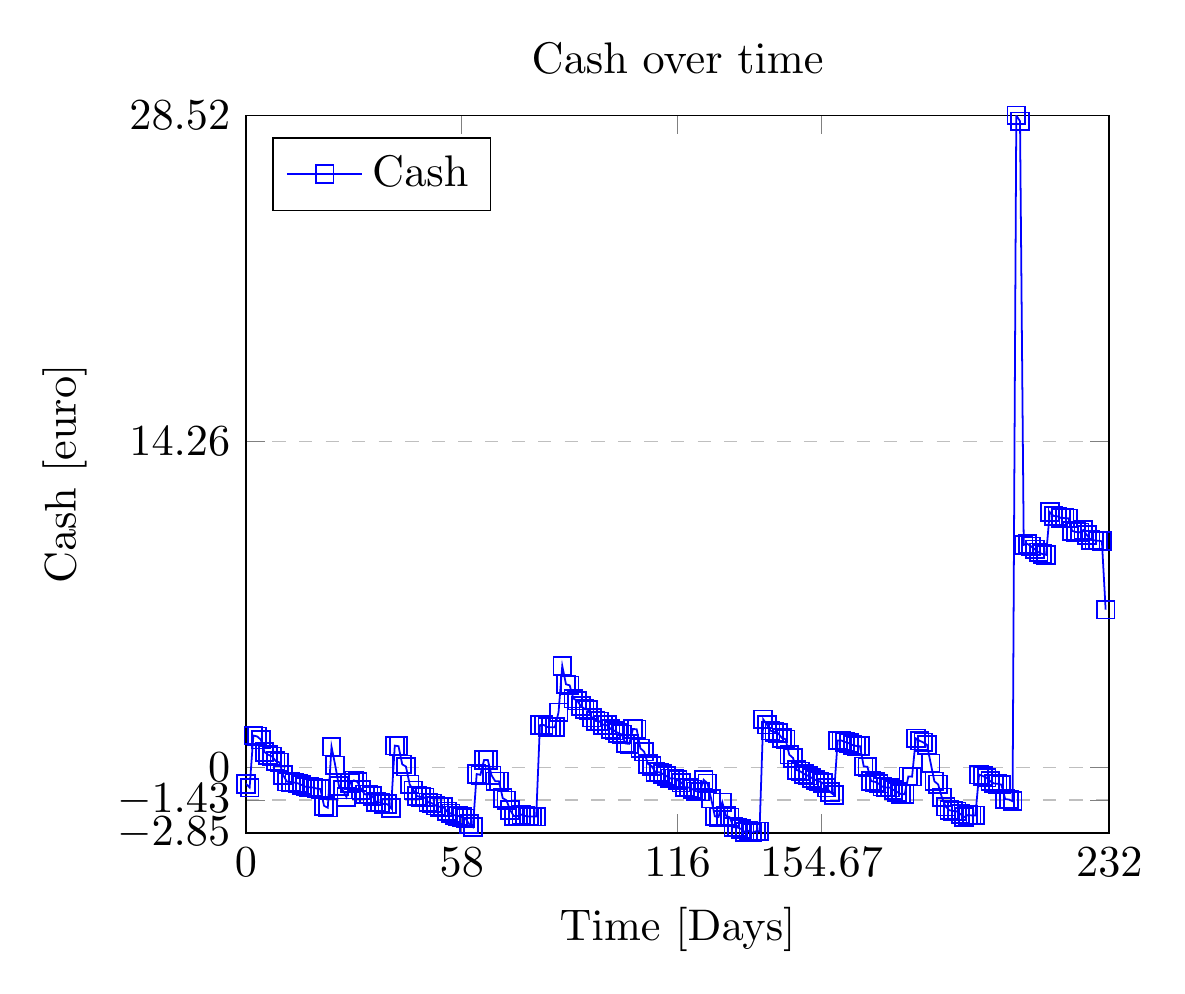
\begin{tikzpicture}[thick, scale=1.6]
\begin{axis}[
title={Cash over time},
xlabel={Time [Days]},
ylabel={Cash [euro]},
xmin=0,xmax=232,
ymin=-2.851,ymax=28.519,
xtick={0,58,116,154.666666666667,232},
ytick={-2.851,-1.4255,0,14.2595,28.519},
legend pos=north west,
ymajorgrids=true,
grid style=dashed,
]
\addplot[
color=blue,
mark=square,
]
coordinates {
(0,-0.713)(1,-0.878)(2,1.4)(3,1.36)(4,1.223)(5,0.676)(6,0.557)(7,0.49)(8,0.285)(9,0.224)(10,-0.329)(11,-0.615)(12,-0.633)(13,-0.658)(14,-0.693)(15,-0.763)(16,-0.841)(17,-0.861)(18,-0.875)(19,-0.918)(20,-0.938)(21,-1.673)(22,-1.757)(23,0.91)(24,0.094)(25,-0.81)(26,-0.968)(27,-1.29)(28,-0.668)(29,-0.563)(30,-0.637)(31,-0.976)(32,-1.175)(33,-1.175)(34,-1.255)(35,-1.51)(36,-1.534)(37,-1.594)(38,-1.603)(39,-1.78)(40,0.959)(41,0.932)(42,0.141)(43,0.04)(44,-0.738)(45,-0.996)(46,-1.25)(47,-1.286)(48,-1.309)(49,-1.52)(50,-1.564)(51,-1.664)(52,-1.719)(53,-1.719)(54,-1.913)(55,-2.009)(56,-2.089)(57,-2.114)(58,-2.164)(59,-2.224)(60,-2.478)(61,-2.605)(62,-0.287)(63,-0.32)(64,0.33)(65,0.33)(66,-0.34)(67,-0.602)(68,-0.606)(69,-1.337)(70,-1.435)(71,-1.858)(72,-2.126)(73,-2.124)(74,-2.06)(75,-2.118)(76,-2.141)(77,-2.147)(78,-2.147)(79,1.853)(80,1.863)(81,1.771)(82,1.757)(83,1.762)(84,2.412)(85,4.446)(86,3.641)(87,3.592)(88,3.015)(89,2.927)(90,2.688)(91,2.568)(92,2.508)(93,2.183)(94,2.039)(95,2.019)(96,1.869)(97,1.849)(98,1.691)(99,1.611)(100,1.51)(101,1.446)(102,1.051)(103,1.036)(104,1.686)(105,1.67)(106,0.841)(107,0.695)(108,0.162)(109,0.067)(110,-0.191)(111,-0.207)(112,-0.28)(113,-0.376)(114,-0.476)(115,-0.476)(116,-0.556)(117,-0.66)(118,-0.867)(119,-0.879)(120,-0.954)(121,-1.04)(122,-1.058)(123,-0.537)(124,-0.688)(125,-1.358)(126,-2.133)(127,-2.161)(128,-1.519)(129,-2.108)(130,-2.176)(131,-2.609)(132,-2.619)(133,-2.679)(134,-2.815)(135,-2.769)(136,-2.851)(137,-2.793)(138,-2.793)(139,2.107)(140,1.873)(141,1.608)(142,1.562)(143,1.501)(144,1.297)(145,1.236)(146,0.563)(147,0.419)(148,-0.11)(149,-0.172)(150,-0.283)(151,-0.359)(152,-0.449)(153,-0.539)(154,-0.601)(155,-0.681)(156,-0.882)(157,-1.071)(158,-1.204)(159,1.181)(160,1.18)(161,1.115)(162,1.064)(163,0.984)(164,0.942)(165,0.933)(166,0.049)(167,0.033)(168,-0.594)(169,-0.624)(170,-0.704)(171,-0.836)(172,-0.871)(173,-0.876)(174,-0.982)(175,-1.075)(176,-1.159)(177,-1.167)(178,-0.389)(179,-0.399)(180,1.273)(181,1.173)(182,1.097)(183,0.991)(184,0.185)(185,-0.604)(186,-0.739)(187,-1.3)(188,-1.709)(189,-1.867)(190,-1.9)(191,-1.918)(192,-2.039)(193,-2.17)(194,-2.079)(195,-2.094)(196,-2.094)(197,-0.31)(198,-0.37)(199,-0.447)(200,-0.599)(201,-0.7)(202,-0.712)(203,-0.748)(204,-1.382)(205,-1.4)(206,-1.473)(207,28.519)(208,28.263)(209,9.736)(210,9.779)(211,9.669)(212,9.538)(213,9.409)(214,9.336)(215,9.302)(216,11.165)(217,11.005)(218,10.987)(219,10.917)(220,10.906)(221,10.901)(222,10.349)(223,10.301)(224,10.284)(225,10.383)(226,10.158)(227,9.954)(228,9.934)(229,9.917)(230,9.896)(231,6.905)
};
\legend{Cash}
\end{axis}
\end{tikzpicture}

\subsection{Incomes}
%Data are aggregated between Initial date: \textbf{2011/01/01} and Last date: \textbf{2021-01-13}

}

\footnotesize{
\subsubsection{Table}
\begin{longtable}{|c|c|c|c|c|}
\hline
\multicolumn{5}{|c|}{Cashflows} \\
\hline
Category & Debit & Credit & PnL \\
\hline
Salary & 0 & 86580 & 86580\\
\hline
Funding & 0 & 42600 & 42600\\
\hline
Cmb & 0 & 7287 & 7287\\
\hline
Bank & 0 & 6097 & 6097\\
\hline
Debt & 0 & 2549 & 2549\\
\hline
Taxes & 0 & 1824 & 1824\\
\hline
Other & 0 & 1191 & 1191\\
\hline
Rent & 0 & 149 & 149\\
\hline
Telephone & 0 & 128 & 128\\
\hline
 ... & ... & ...\\
\hline
 Total & 140420 & 142872 & 2452 \\
\hline
\end{longtable}

\subsubsection{Graph}
\begin{bchart}[min=0,max=86,step=17,unit=k\texteuro]
\bcbar[label=Salary]{86}\\
\smallskip
\bcbar[label=Funding]{42}\\
\smallskip
\bcbar[label=Cmb]{7}\\
\smallskip
\bcbar[label=Bank]{6}\\
\smallskip
\bcbar[label=Debt]{2}\\
\smallskip
\bcbar[label=Taxes]{1}\\
\smallskip
\bcbar[label=Other]{1}\\
\smallskip
\bcbar[label=Rent]{0}\\
\smallskip
\bcbar[label=Telephone]{0}\\
\smallskip
\end{bchart}

\subsubsection{Chart}
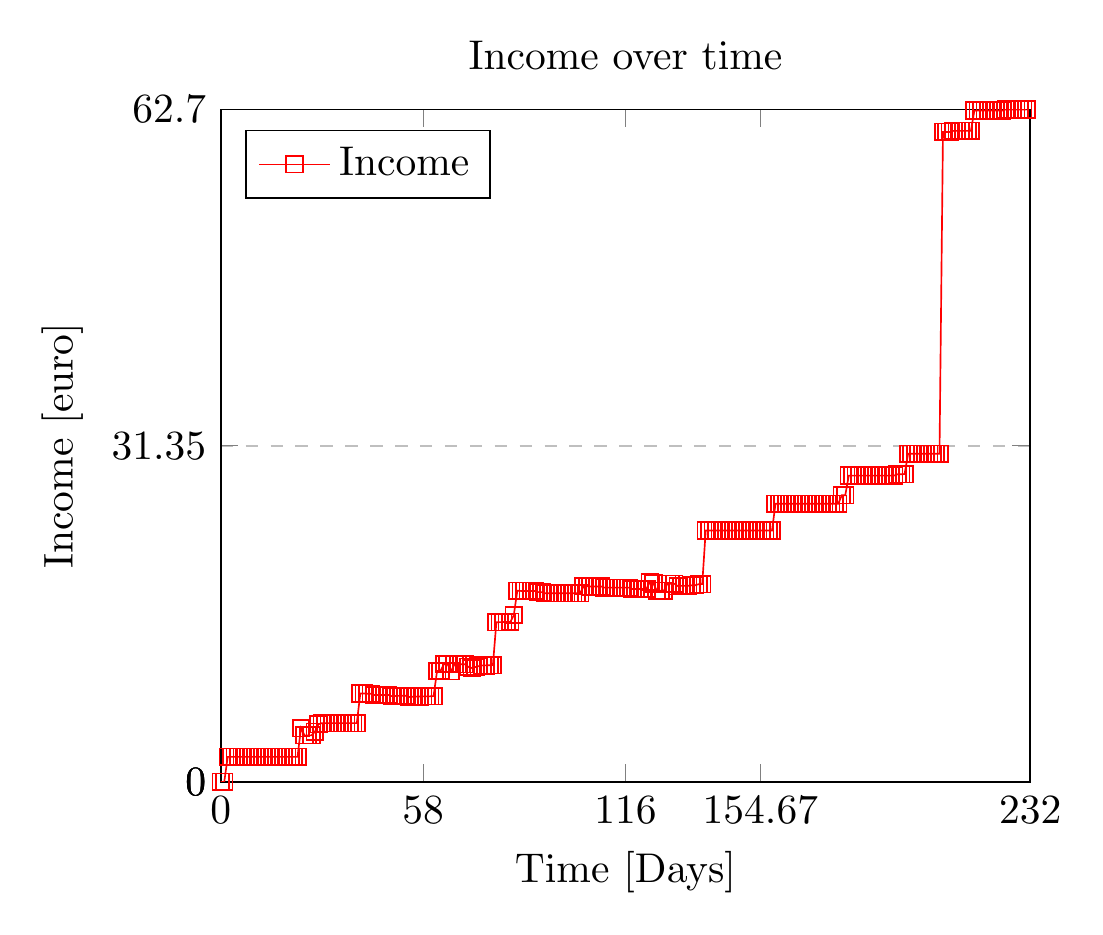
\begin{tikzpicture}[thick, scale=1.5]
\begin{axis}[
title={Income over time},
xlabel={Time [Days]},
ylabel={Income [euro]},
xmin=0,xmax=232,
ymin=0,ymax=62.704,
xtick={0,58,116,154.666666666667,232},
ytick={0,0,0,31.352,62.704},
legend pos=north west,
ymajorgrids=true,
grid style=dashed,
]
\addplot[
color=red,
mark=square,
]
coordinates {
(0,0)(1,0)(2,2.34)(3,2.34)(4,2.34)(5,2.34)(6,2.34)(7,2.34)(8,2.34)(9,2.34)(10,2.34)(11,2.34)(12,2.34)(13,2.34)(14,2.34)(15,2.34)(16,2.34)(17,2.34)(18,2.34)(19,2.34)(20,2.34)(21,2.34)(22,2.34)(23,5.015)(24,4.345)(25,4.345)(26,4.345)(27,4.68)(28,5.38)(29,5.485)(30,5.485)(31,5.485)(32,5.485)(33,5.485)(34,5.485)(35,5.485)(36,5.485)(37,5.485)(38,5.485)(39,5.485)(40,8.248)(41,8.248)(42,8.228)(43,8.228)(44,8.102)(45,8.112)(46,8.112)(47,8.112)(48,8.112)(49,8.002)(50,8.01)(51,8.026)(52,8.034)(53,8.034)(54,7.925)(55,7.941)(56,7.957)(57,7.965)(58,7.981)(59,7.981)(60,7.981)(61,8.005)(62,10.345)(63,10.345)(64,10.995)(65,10.995)(66,10.325)(67,10.975)(68,10.975)(69,10.975)(70,10.975)(71,10.724)(72,10.621)(73,10.713)(74,10.803)(75,10.865)(76,10.865)(77,10.881)(78,10.889)(79,14.889)(80,14.899)(81,14.91)(82,14.91)(83,14.916)(84,15.566)(85,17.83)(86,17.81)(87,17.81)(88,17.81)(89,17.81)(90,17.81)(91,17.7)(92,17.7)(93,17.596)(94,17.596)(95,17.596)(96,17.596)(97,17.596)(98,17.596)(99,17.596)(100,17.596)(101,17.596)(102,17.596)(103,17.596)(104,18.246)(105,18.246)(106,18.226)(107,18.226)(108,18.226)(109,18.226)(110,18.116)(111,18.116)(112,18.116)(113,18.116)(114,18.116)(115,18.116)(116,18.116)(117,18.116)(118,17.99)(119,17.99)(120,17.99)(121,17.99)(122,17.99)(123,18.64)(124,18.497)(125,17.827)(126,17.827)(127,17.827)(128,18.477)(129,18.477)(130,18.477)(131,18.264)(132,18.28)(133,18.28)(134,18.288)(135,18.334)(136,18.342)(137,18.44)(138,18.448)(139,23.448)(140,23.448)(141,23.448)(142,23.448)(143,23.448)(144,23.448)(145,23.448)(146,23.448)(147,23.448)(148,23.448)(149,23.448)(150,23.448)(151,23.448)(152,23.448)(153,23.448)(154,23.448)(155,23.448)(156,23.448)(157,23.448)(158,23.448)(159,25.937)(160,25.937)(161,25.937)(162,25.937)(163,25.937)(164,25.937)(165,25.937)(166,25.937)(167,25.937)(168,25.937)(169,25.937)(170,25.937)(171,25.937)(172,25.937)(173,25.937)(174,25.937)(175,25.937)(176,25.937)(177,25.937)(178,26.737)(179,26.737)(180,28.562)(181,28.562)(182,28.562)(183,28.562)(184,28.562)(185,28.562)(186,28.562)(187,28.562)(188,28.562)(189,28.562)(190,28.562)(191,28.562)(192,28.562)(193,28.565)(194,28.685)(195,28.693)(196,28.709)(197,30.605)(198,30.605)(199,30.605)(200,30.605)(201,30.605)(202,30.605)(203,30.605)(204,30.605)(205,30.605)(206,30.605)(207,60.605)(208,60.605)(209,60.605)(210,60.704)(211,60.704)(212,60.704)(213,60.704)(214,60.704)(215,60.704)(216,62.595)(217,62.6)(218,62.6)(219,62.6)(220,62.6)(221,62.6)(222,62.6)(223,62.6)(224,62.6)(225,62.704)(226,62.704)(227,62.704)(228,62.704)(229,62.704)(230,62.704)(231,62.704)
};
\legend{Income}
\end{axis}
\end{tikzpicture}

%\includegraphics[width=.8\textwidth]{Income.png}
}

\subsection{Charges}
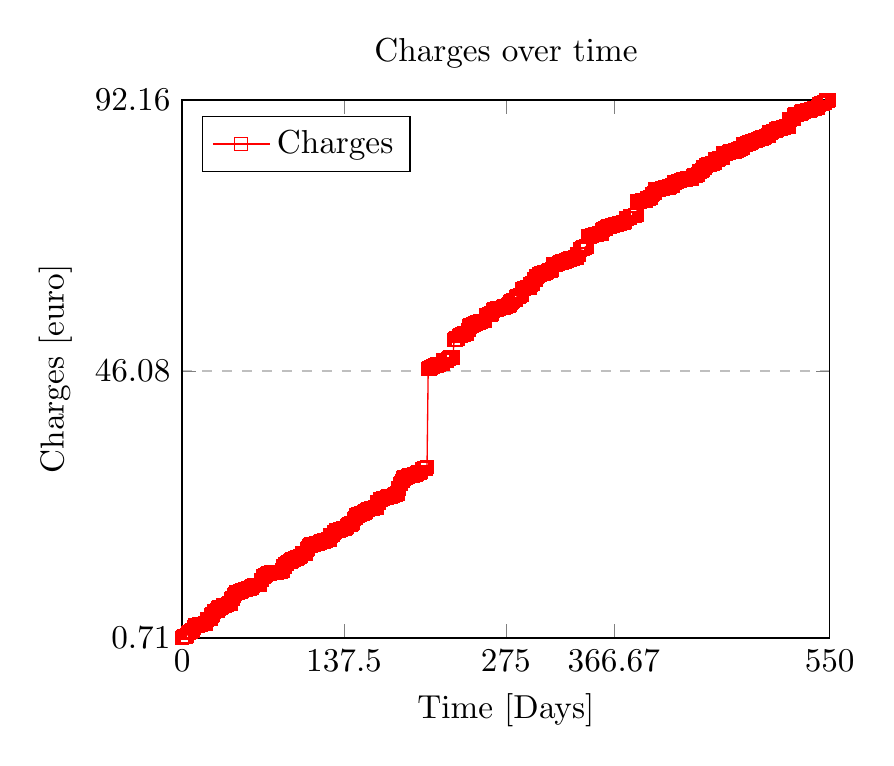
\begin{tikzpicture}[thick, scale=1.2]
\begin{axis}[
title={Charges over time},
xlabel={Time [Days]},
ylabel={Charges [euro]},
xmin=0,xmax=550,
ymin=0.713,ymax=92.162,
xtick={0,137.5,275,366.666666666667,550},
ytick={0.713,0.3565,0,46.081,92.162},
legend pos=north west,
ymajorgrids=true,
grid style=dashed,
]
\addplot[
color=red,
mark=square,
]
coordinates {
(0,0.713)(1,0.878)(2,0.94)(3,0.98)(4,1.117)(5,1.518)(6,1.637)(7,1.704)(8,1.909)(9,1.97)(10,2.523)(11,2.809)(12,2.827)(13,2.852)(14,2.887)(15,2.957)(16,3.035)(17,3.055)(18,3.069)(19,3.112)(20,3.132)(21,3.855)(22,3.939)(23,3.947)(24,3.957)(25,4.526)(26,4.684)(27,5.195)(28,5.273)(29,5.273)(30,5.347)(31,5.686)(32,5.885)(33,5.885)(34,5.965)(35,6.22)(36,6.244)(37,6.304)(38,6.313)(39,6.49)(40,6.514)(41,6.541)(42,7.312)(43,7.413)(44,7.915)(45,8.183)(46,8.437)(47,8.473)(48,8.496)(49,8.597)(50,8.649)(51,8.765)(52,8.828)(53,8.828)(54,8.913)(55,9.025)(56,9.121)(57,9.154)(58,9.22)(59,9.28)(60,9.534)(61,9.685)(62,9.707)(63,9.74)(64,9.74)(65,9.74)(66,9.74)(67,10.551)(68,10.555)(69,11.14)(70,11.238)(71,11.41)(72,11.575)(73,11.621)(74,11.647)(75,11.767)(76,11.79)(77,11.812)(78,11.82)(79,11.82)(80,11.82)(81,11.885)(82,11.899)(83,11.9)(84,11.9)(85,12.13)(86,12.814)(87,12.863)(88,13.294)(89,13.382)(90,13.621)(91,13.631)(92,13.691)(93,13.912)(94,14.056)(95,14.076)(96,14.226)(97,14.246)(98,14.404)(99,14.484)(100,14.585)(101,14.649)(102,15.044)(103,15.059)(104,15.059)(105,15.075)(106,15.783)(107,15.929)(108,16.316)(109,16.411)(110,16.559)(111,16.575)(112,16.603)(113,16.699)(114,16.799)(115,16.799)(116,16.879)(117,16.983)(118,17.064)(119,17.076)(120,17.151)(121,17.237)(122,17.255)(123,17.384)(124,17.392)(125,17.392)(126,18.167)(127,18.195)(128,18.203)(129,18.646)(130,18.714)(131,18.934)(132,18.96)(133,19.02)(134,19.164)(135,19.164)(136,19.254)(137,19.294)(138,19.302)(139,19.402)(140,19.636)(141,19.901)(142,19.947)(143,20.008)(144,20.212)(145,20.273)(146,20.946)(147,21.09)(148,21.473)(149,21.535)(150,21.646)(151,21.722)(152,21.812)(153,21.902)(154,21.964)(155,22.044)(156,22.245)(157,22.434)(158,22.521)(159,22.625)(160,22.626)(161,22.691)(162,22.742)(163,22.822)(164,22.864)(165,22.873)(166,23.75)(167,23.766)(168,24.234)(169,24.264)(170,24.344)(171,24.476)(172,24.507)(173,24.512)(174,24.618)(175,24.711)(176,24.795)(177,24.803)(178,24.825)(179,24.835)(180,24.988)(181,25.088)(182,25.164)(183,25.27)(184,26.076)(185,26.865)(186,27)(187,27.415)(188,27.824)(189,27.982)(190,28.015)(191,28.033)(192,28.154)(193,28.288)(194,28.317)(195,28.34)(196,28.356)(197,28.468)(198,28.528)(199,28.605)(200,28.757)(201,28.858)(202,28.87)(203,28.906)(204,29.394)(205,29.412)(206,29.485)(207,29.493)(208,29.749)(209,46.441)(210,46.497)(211,46.607)(212,46.738)(213,46.867)(214,46.94)(215,46.974)(216,47.002)(217,47.167)(218,47.185)(219,47.255)(220,47.266)(221,47.271)(222,47.823)(223,47.868)(224,47.885)(225,47.89)(226,48.11)(227,48.314)(228,48.334)(229,48.351)(230,48.37)(231,51.361)(232,51.439)(233,51.556)(234,51.584)(235,52.034)(236,52.1)(237,52.12)(238,52.236)(239,52.315)(240,52.455)(241,52.46)(242,52.508)(243,53.029)(244,53.692)(245,53.797)(246,53.839)(247,53.969)(248,53.982)(249,54.177)(250,54.261)(251,54.299)(252,54.306)(253,54.533)(254,54.545)(255,54.575)(256,54.586)(257,54.594)(258,55.6)(259,55.615)(260,55.63)(261,55.722)(262,55.729)(263,55.872)(264,56.413)(265,56.497)(266,56.504)(267,56.515)(268,56.716)(269,56.745)(270,56.776)(271,56.784)(272,56.81)(273,56.899)(274,57.011)(275,57.035)(276,57.126)(277,57.264)(278,57.383)(279,57.775)(280,57.94)(281,58.015)(282,58.121)(283,58.137)(284,58.653)(285,58.725)(286,58.748)(287,58.933)(288,59.013)(289,60.024)(290,60.031)(291,60.165)(292,60.17)(293,60.257)(294,60.262)(295,60.266)(296,60.831)(297,60.926)(298,60.964)(299,61.617)(300,61.623)(301,62.154)(302,62.254)(303,62.467)(304,62.537)(305,62.692)(306,62.7)(307,62.7)(308,62.835)(309,62.845)(310,62.925)(311,63.066)(312,63.124)(313,63.197)(314,63.302)(315,64.179)(316,64.207)(317,64.233)(318,64.242)(319,64.278)(320,64.468)(321,64.523)(322,64.571)(323,64.671)(324,64.713)(325,64.737)(326,64.863)(327,64.892)(328,65.025)(329,65.071)(330,65.185)(331,65.189)(332,65.219)(333,65.283)(334,65.335)(335,65.359)(336,65.875)(337,65.918)(338,66.728)(339,66.841)(340,66.868)(341,67.031)(342,67.06)(343,67.221)(344,67.261)(345,68.937)(346,68.947)(347,69.003)(348,69.075)(349,69.201)(350,69.213)(351,69.238)(352,69.25)(353,69.356)(354,69.404)(355,69.436)(356,69.444)(357,70.018)(358,70.188)(359,70.263)(360,70.322)(361,70.587)(362,70.595)(363,70.655)(364,70.71)(365,70.792)(366,70.838)(367,70.926)(368,70.933)(369,70.956)(370,71.068)(371,71.183)(372,71.189)(373,71.233)(374,71.252)(375,71.312)(376,71.433)(377,71.982)(378,72.006)(379,72.082)(380,72.113)(381,72.417)(382,72.438)(383,72.446)(384,72.454)(385,72.623)(386,72.63)(387,74.853)(388,74.864)(389,74.88)(390,74.956)(391,75.054)(392,75.061)(393,75.068)(394,75.076)(395,75.375)(396,75.428)(397,75.518)(398,75.544)(399,76.084)(400,76.184)(401,76.357)(402,76.888)(403,76.93)(404,76.939)(405,76.951)(406,77.018)(407,77.044)(408,77.134)(409,77.216)(410,77.223)(411,77.246)(412,77.278)(413,77.308)(414,77.484)(415,77.558)(416,77.581)(417,77.588)(418,78.101)(419,78.201)(420,78.212)(421,78.356)(422,78.364)(423,78.378)(424,78.554)(425,78.575)(426,78.585)(427,78.598)(428,78.622)(429,78.753)(430,78.77)(431,78.793)(432,78.797)(433,78.837)(434,79.243)(435,79.302)(436,79.341)(437,79.431)(438,79.496)(439,80.015)(440,80.022)(441,80.09)(442,80.261)(443,80.683)(444,80.708)(445,81.047)(446,81.109)(447,81.198)(448,81.233)(449,81.301)(450,81.308)(451,81.356)(452,81.435)(453,81.984)(454,82.009)(455,82.048)(456,82.16)(457,82.268)(458,82.281)(459,82.288)(460,83.013)(461,83.05)(462,83.057)(463,83.134)(464,83.137)(465,83.313)(466,83.384)(467,83.406)(468,83.414)(469,83.437)(470,83.52)(471,83.588)(472,83.696)(473,83.714)(474,83.87)(475,83.99)(476,84.006)(477,84.544)(478,84.559)(479,84.628)(480,84.784)(481,84.791)(482,84.917)(483,84.947)(484,85.14)(485,85.164)(486,85.179)(487,85.286)(488,85.375)(489,85.472)(490,85.523)(491,85.583)(492,85.587)(493,85.796)(494,85.811)(495,85.844)(496,86.006)(497,86.031)(498,86.1)(499,86.609)(500,86.638)(501,86.706)(502,86.858)(503,86.884)(504,86.906)(505,87.088)(506,87.335)(507,87.343)(508,87.354)(509,87.383)(510,87.41)(511,87.473)(512,87.578)(513,87.6)(514,87.625)(515,87.638)(516,88.826)(517,88.932)(518,88.936)(519,88.947)(520,89.629)(521,89.637)(522,89.722)(523,89.746)(524,89.775)(525,89.797)(526,89.99)(527,90.235)(528,90.242)(529,90.251)(530,90.26)(531,90.325)(532,90.37)(533,90.405)(534,90.536)(535,90.585)(536,90.612)(537,90.749)(538,90.785)(539,90.812)(540,90.859)(541,91.388)(542,91.434)(543,91.556)(544,91.576)(545,91.746)(546,91.753)(547,92.035)(548,92.067)(549,92.162)
};
\legend{Charges}
\end{axis}
\end{tikzpicture}


\subsubsection{Charges plot}
\includegraphics[scale=0.3]{Charges2.png}

\subsubsection{Charges kiviat}
\begin{tikzpicture}[scale=0.5]
\tkzKiviatDiagramFromFile[
        scale=.5,
        label distance=.5cm,
        gap     = 1,
        label space=3,  
        lattice = 10]{chargesKiviat.dat}
\tkzKiviatLineFromFile[thick,
                       color      = blue,
                       mark       = ball,
                       ball color = blue,
                       mark size  = 4pt,
                       fill       = blue!20]{chargesKiviat.dat}{2}
\tkzKiviatLineFromFile[thick,
                       color      = red,
                       mark       = ball,
                       ball color = red,
                       mark size  = 4pt,
                       fill       = red!20]{chargesKiviat.dat}{1}     
\end{tikzpicture}


\subsubsection{Table}
\begin{longtable}{|c|c|c|c|c|}
\hline
\multicolumn{5}{|c|}{Cashflows} \\
\hline
Category & Debit & Credit & PnL \\
\hline
Cmb & 7201 & -963 & -8164\\
\hline
Debt & 19965 & 0 & -19965\\
\hline
Bank & 8527 & 0 & -8527\\
\hline
Other & 8205 & 0 & -8205\\
\hline
Cash & 4330 & 0 & -4330\\
\hline
Food & 2487 & 0 & -2487\\
\hline
Toxics & 2395 & 0 & -2395\\
\hline
Rent & 1066 & 0 & -1066\\
\hline
Telephone & 669 & 0 & -669\\
\hline
Energy & 448 & 0 & -448\\
\hline
Home & 272 & 0 & -272\\
\hline
Health & 232 & 0 & -232\\
\hline
Transport & 2 & 0 & -2\\
\hline
 ... & ... & ... & ...\\
\hline
 Total & 55799 & 62704 & 6905 \\
\hline
\end{longtable}


\subsubsection{Graph}
\begin{bchart}[min=0,max=19,step=3,unit=k\texteuro]
\bcbar[label=Cmb]{7}\\
\smallskip
\bcbar[label=Debt]{19}\\
\smallskip
\bcbar[label=Bank]{8}\\
\smallskip
\bcbar[label=Other]{8}\\
\smallskip
\bcbar[label=Cash]{4}\\
\smallskip
\bcbar[label=Food]{2}\\
\smallskip
\bcbar[label=Toxics]{2}\\
\smallskip
\bcbar[label=Rent]{1}\\
\smallskip
\bcbar[label=Telephone]{0}\\
\smallskip
\bcbar[label=Energy]{0}\\
\smallskip
\bcbar[label=Home]{0}\\
\smallskip
\bcbar[label=Health]{0}\\
\smallskip
\bcbar[label=Transport]{0}\\
\smallskip
\end{bchart}


\subsubsection{Chart}

\subsubsection{Cheese}
\begin{tikzpicture}[scale=3]
\foreach \p/\t in {
12 / Cmb-7.201k\texteuro ,
35 / Debt-19.965k\texteuro ,
15 / Bank-8.527k\texteuro ,
14 / Other-8.205k\texteuro ,
7 / Cash-4.33k\texteuro ,
4 / Food-2.487k\texteuro ,
4 / Toxics-2.395k\texteuro ,
1 / Rent-1.066k\texteuro ,
1 / Telephone-0.669k\texteuro ,
0 / Energy-0.448k\texteuro 
0 / Home-0.272k\texteuro 
0 / Health-0.232k\texteuro 
0 / Transport-0.002k\texteuro 
}
  {
\setcounter{a}{\value{b}}
\addtocounter{b}{\p}
\slice{\thea/100*360}
          {\theb/100*360}
          {\p\%}{\t}
  }
\end{tikzpicture}


\section{Asset Liability Management}

\subsection{Kapital}

\subsubsection{Table}
History of the Kapital is available in the database (select * from kapital)

%$\lim_{x \to \infty} \exp(-x) = 0$
%$\lim_{x \to \infty} \exp(-x) = 0$
%K: Kapital\\
%A: Assets\\
%L: Liabilities\\
%K = A-L\\
%L = K/L\\

\subsubsection{Graph}
A graph of the kapital and not income and charges cumulated should be easy to build.
Say a readKapital which would select the cash balance + all the other stuff like assets - liabilities
Better do it with Latex than with the C++ 

\subsubsection{History}
{\footnotesize
Historical graph of the kapital, liab and assets, yearly ALM management\\
%\includegraphics[width=.8\textwidth]{Assets.png}
}

\subsubsection{Definitions}
{\footnotesize
Vp: value weight (basically the value of the asset against the total value - to be replaced by InitPrice)\\
Rp: return weight (the return compared to the total returns)\\
Cp: cost weight (the maintenance cost compared to the total maintenance\\
Vd: historical deprecation of value (the Value compared to the InitPrice\\
R/V: monthly rentability (the return minus the maintenance)\\}

\subsubsection{Ratios}
{\footnotesize
Vp = value/Totalvalue\\
Rp = return/Totalreturn\\
Cp = cost/Totalmaintenance\\
Vd = value/Initprice\\
R/V = return/Value\\}

\subsubsection{Formulas}

{\footnotesize
%$\lim_{x \to \infty} \exp(-x) = 0$\\
}

\subsection{Assets}

\subsubsection{Data}
The top 5 assets are listed sorted by value, but the totals are given for all the assets as of today\\

\begin{longtable}{|c|c|c|c|c|c|c|c|c|c|c|c|}
\hline
\multicolumn{12}{|c|}{Assets} \\
\hline
Type & Name & Maturity & Value & Return & Cost & InitPrice & vp & rp & mp & dv & PnL(R/V)\\
\hline
Boat & Acquisition & 2013-01-07 & 17000 & 50 & 400 & 30000 & 72 & 0 & 3 & 56 & 0\\
\hline
CEL & Acquisition & 2013-01-07 & 483 & 50 & 400 & 30000 & 2 & 0 & 3 & 1 & 0\\
\hline
LDD & Acquisition & 2013-01-07 & 42 & 50 & 400 & 30000 & 0 & 0 & 3 & 0 & 0\\
\hline
TITR & Acquisition & 2013-01-07 & 47 & 50 & 400 & 30000 & 0 & 0 & 3 & 0 & 0\\
\hline
PRED & Acquisition & 2013-01-07 & 140 & 50 & 400 & 30000 & 0 & 0 & 3 & 0 & 0\\
\hline
 ... & ... & ... & ... & ... & ... & ... & ... & ... & ... & ... & ...\\
\hline
& Total assets & 272834 & 23408 & 7991 & 10267 & & & & & & -2276\\
\hline
\end{longtable}


\subsubsection{Graph}
\begin{bchart}[min=0,max=17,step=3,unit=k\texteuro]
\bcbar[label=Boat]{17}\\
\smallskip
\bcbar[label=Alfa]{3}\\
\smallskip
\bcbar[label=Guitars]{0.35}\\
\smallskip
\bcbar[label=Tvsamsung]{0.49}\\
\smallskip
\bcbar[label=Motor]{0.5}\\
\smallskip
\end{bchart}
;

\subsubsection{Cheese}
\begin{tikzpicture}[scale=2]
\foreach \p/\t in {
72 / Boat-17k\texteuro -0\ ,
12 / Alfa-3k\texteuro -0\ ,
1 / Guitars-0.35k\texteuro -0\ ,
2 / Tvsamsung-0.49k\texteuro -0\ ,
2 / Motor-0.5k\texteuro -0\i ,
}
  {
\setcounter{a}{\value{b}}
\addtocounter{b}{\p}
\slice{\thea/100*360}
          {\theb/100*360}
          {\p\%}{\t}
  }
\end{tikzpicture}


\subsubsection{Kiviat}
\input{assetsKiviat}
Seems like the assets Cheese 

\subsection{Liabilities}
The top 4 liabilities are listed but the totals are given for all the liabilities\\

\footnotesize{
\subsubsection{Table}
\begin{longtable}{|c|c|c|c|c|c|c|c|c|c|c|c|}
\hline
\multicolumn{12}{|c|}{Liabilities} \\
\hline
Type & Name & InitPrice & Value & Return & Cost & Maturity & vp & rp & mp & dv & PnL\\
\hline
Boat-mortgage & mortgage & 30000 & 13440 & 0 & 1 & 2013-01-07 & 55 & 0 & 25 & 44 & 0\\
\hline
Car-mortgage & mortgage & 7000 & 2287 & 0 & 1 & 2013-01-07 & 9 & 0 & 25 & 32 & 0\\
\hline
Dad-mortgage & mortgage & 5000 & 5000 & 0 & 1 & 2013-01-07 & 20 & 0 & 25 & 100 & 0\\
\hline
Mum-mortgage & mortgage & 3500 & 3500 & 0 & 1 & 2013-01-07 & 14 & 0 & 25 & 100 & 0\\
\hline
 ... & ... & ... & ... & ... & ... & ... & ... & ... & ... & ... & ...\\
\hline
& Total & 45500 & 24227 & 0 & 4 & & & & & & -4\\
\hline
\end{longtable}

\subsubsection{Graph}
\begin{bchart}[min=0,max=13,step=2,unit=k\texteuro]
\bcbar[label=Boat-mortgage]{13.44}\\
\smallskip
\bcbar[label=Car-mortgage]{2.287}\\
\smallskip
\bcbar[label=Dad-mortgage]{5}\\
\smallskip
\bcbar[label=Mum-mortgage]{3.5}\\
\smallskip
\end{bchart}

\subsubsection{Chart}
%\includegraphics[width=.8\textwidth]{Liabilities.png}
\subsubsection{Cheese}
\begin{tikzpicture}[scale=2]
\foreach \p/\t in {
55 / Boat-mortgage- 13 k\texteuro ,
9 / Car-mortgage- 2 k\texteuro ,
20 / Dad-mortgage- 5 k\texteuro ,
14 / Mum-mortgage- 3 k\texteuro ,
}
  {
\setcounter{a}{\value{b}}
\addtocounter{b}{\p}
\slice{\thea/100*360}
          {\theb/100*360}
          {\p\%}{\t}
  }
\end{tikzpicture}

}

\section{Cashflows}

%\subsection{Management summary}

\footnotesize{
All cashflows from history are being used here\\
}

{\footnotesize
\subsubsection{Table}
\begin{longtable}{|c|c|c|c|c|}
\hline
\multicolumn{5}{|c|}{Cashflows} \\
\hline
Category & Debit & Credit & PnL \\
\hline
Other & 0.0000001 & 0.0000001 & 0\\
\hline
Other & 104 & 0 & -104\\
\hline
Other & 13 & 0 & -13\\
\hline
Other & 10 & 0 & -10\\
\hline
Other & 190 & 0 & -190\\
\hline
Other & 8 & 0 & -8\\
\hline
Other & 16 & 0 & -16\\
\hline
Other & 4 & 0 & -4\\
\hline
Other & 6 & 0 & -6\\
\hline
Other & 14 & 0 & -14\\
\hline
 ... & ... & ... & ...\\
\hline
 Total & 112143.00006290044 & 117930.00006290042 & 5786.99999999999 \\
\hline
\end{longtable}

\subsubsection{Graph}
%\begin{bchart}[min=0,max=11214,step=3738,unit=k\texteuro]
\bcbar[label=Other]{0}\\
\smallskip
\bcbar[label=Other]{10}\\
\smallskip
\bcbar[label=Other]{1}\\
\smallskip
\bcbar[label=Other]{1}\\
\smallskip
\bcbar[label=Other]{19}\\
\smallskip
\bcbar[label=Other]{0}\\
\smallskip
\bcbar[label=Other]{1}\\
\smallskip
\bcbar[label=Other]{0}\\
\smallskip
\bcbar[label=Other]{0}\\
\smallskip
\bcbar[label=Other]{1}\\
\smallskip
\end{bchart}

}

\section{Stocks}

%\subsection{Management summary}

\footnotesize{
All stocks and the evolution of their stock price are shown here\\
}

{\footnotesize
\subsubsection{Table}
Stocks table is available in the database ;-)
select * from stocks
%\begin{longtable}{|c|c|c|c|c|}
\hline
\multicolumn{5}{|c|}{Cashflows} \\
\hline
Category & Debit & Credit & PnL \\
\hline
Other & 0.0000001 & 0.0000001 & 0\\
\hline
Other & 104 & 0 & -104\\
\hline
Other & 13 & 0 & -13\\
\hline
Other & 10 & 0 & -10\\
\hline
Other & 190 & 0 & -190\\
\hline
Other & 8 & 0 & -8\\
\hline
Other & 16 & 0 & -16\\
\hline
Other & 4 & 0 & -4\\
\hline
Other & 6 & 0 & -6\\
\hline
Other & 14 & 0 & -14\\
\hline
 ... & ... & ... & ...\\
\hline
 Total & 112143.00006290044 & 117930.00006290042 & 5786.99999999999 \\
\hline
\end{longtable}

\subsubsection{Graph}
The graph is also available and produced by C++ under "legends"
%\begin{bchart}[min=0,max=11214,step=3738,unit=k\texteuro]
\bcbar[label=Other]{0}\\
\smallskip
\bcbar[label=Other]{10}\\
\smallskip
\bcbar[label=Other]{1}\\
\smallskip
\bcbar[label=Other]{1}\\
\smallskip
\bcbar[label=Other]{19}\\
\smallskip
\bcbar[label=Other]{0}\\
\smallskip
\bcbar[label=Other]{1}\\
\smallskip
\bcbar[label=Other]{0}\\
\smallskip
\bcbar[label=Other]{0}\\
\smallskip
\bcbar[label=Other]{1}\\
\smallskip
\end{bchart}

%\includepdf[pages={1}]{stockchart.pdf}
}

\end{document}

\end{document}
